\documentclass[12pt,a4paper]{article}
\usepackage{graphicx}
\usepackage{amsmath}
\usepackage{bm}
\usepackage{interval}
\usepackage{amssymb}
\usepackage{float}
\usepackage{subfigure}
\usepackage[letterpaper,top=2cm,bottom=2cm,left=3cm,right=3cm,marginparwidth=1.75cm]{geometry}
\usepackage[colorlinks=true, allcolors=blue]{hyperref}

\title{ICN Programming Assignment Report 1}
\author{Student ID: b10201054}

\begin{document}
\maketitle

\section{TCP transmission}

\subsection{socket\_client}
First, we look at socket\_client.py. In the Figure 1.(a), we set up the HOST and PORT of client then build a socket.
In the Figure 2.(b), we first receive the msg from server, since the msg is encoded by utf-8, we need to decode it to get the msg.
Then, we send the question we want to ask with encoding by utf-8. Last, we receive the msg from server again to get the ans.
The if block is to send the response to server prompt.
\begin{figure}[H]
    \centering
    \subfigure[set HOST, PORT]{
        \label{Fig.sub.1-1}
        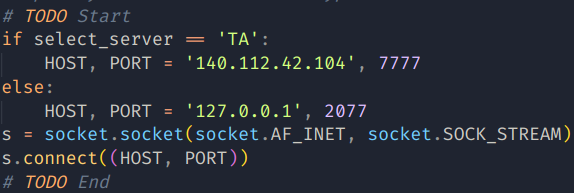
\includegraphics[width = 0.48\linewidth]{P1-1.png}    
    }\subfigure[send msg to server]{
        \label{Fig.sub.1-2}
        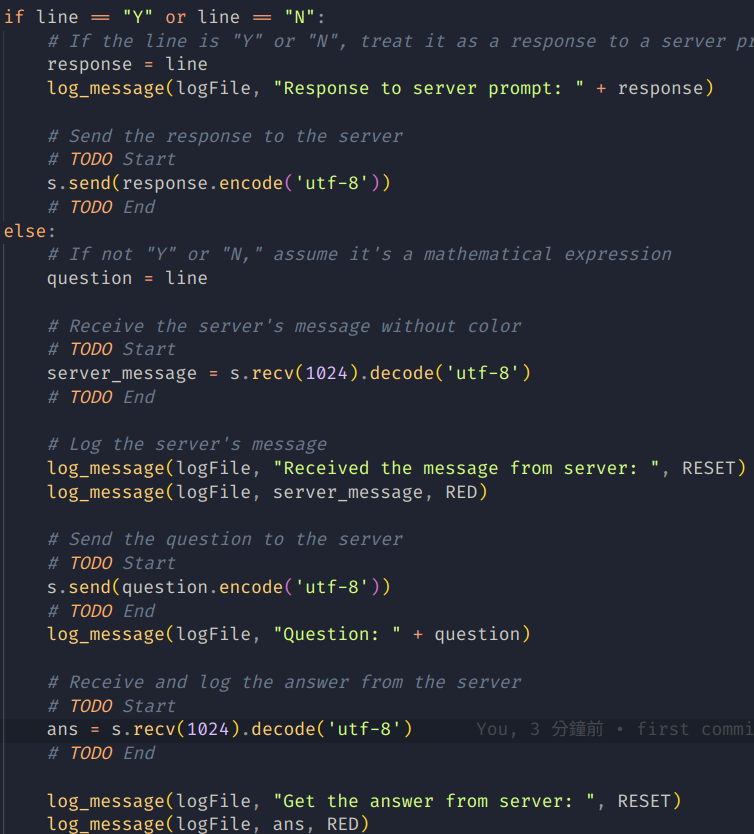
\includegraphics[width = 0.48\linewidth]{P1-2.png}
    }
    \caption{Socket\_client.py}
\end{figure}

\subsection{socket\_server}
The settings of HOST, PORT, socket are same as client part, the unique step is to listen the channel in Figure 2.(b). 
Listen function is to tell server how much request it can handle simultaneously. 
Accept function is to get the client's socket and its address.
In the Figure 2.(c), send and receive are same as client part. 
\begin{figure}[H]
    \centering
    \subfigure[set HOST, PORT, socket]{
        \label{Fig.sub.1-3}
        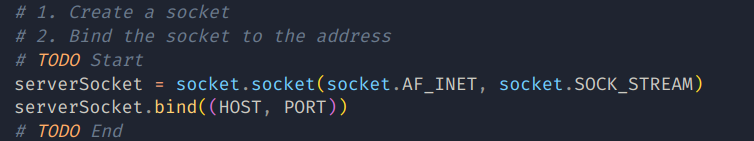
\includegraphics[width = 0.48\linewidth]{P1-3.png}    
    }\subfigure[accept the link from client]{
        \label{Fig.sub.1-4}
        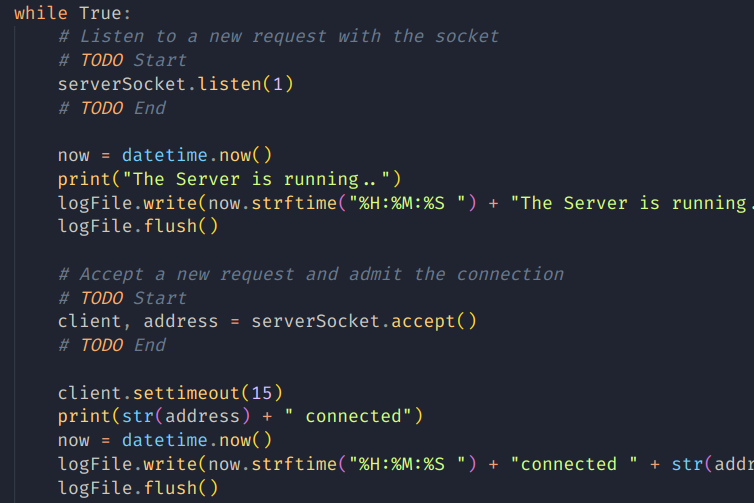
\includegraphics[width = 0.48\linewidth]{P1-4.png}
    }
    \subfigure[send and receive]{
        \label{Fig.sub.1-5}
        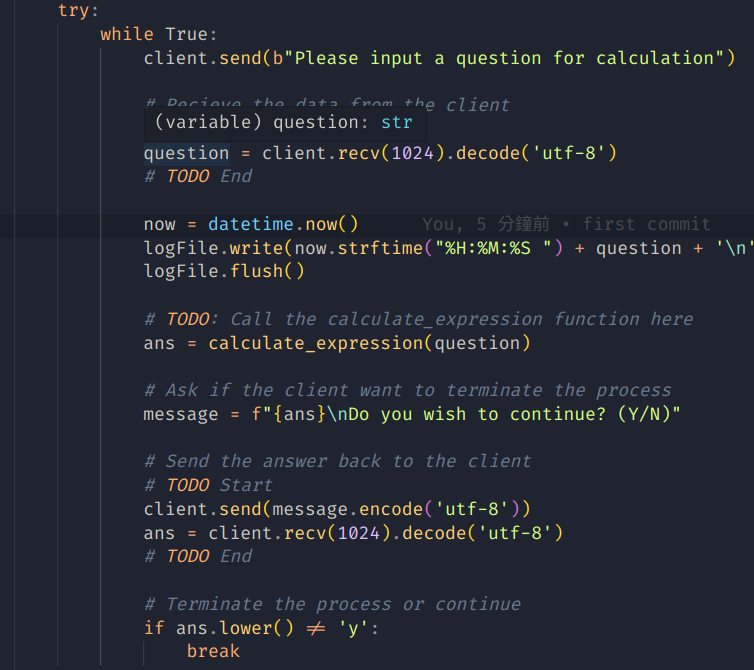
\includegraphics[width = 0.48\linewidth]{P1-5.png}
    }\subfigure[Final result at client side]{
        \label{Fig.sub.1-6}
        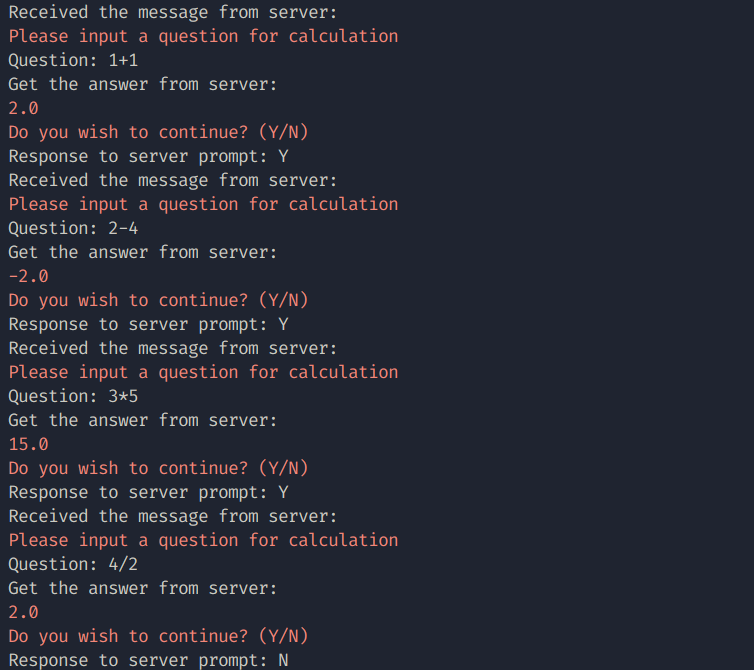
\includegraphics[width = 0.48\linewidth]{P1-final.png}
    }
    \caption{Socket\_server.py}
\end{figure}
\newpage
\section{HTTP server}    
\subsection{Code}
In Figure 3.(a)and(b), we do the same thing as socket\_server to establish a socket.
In Figure 3.(c), we split the msg to get the filename the client wants.
In Figure 3.(d), if we can open the file the client asks, we send http response 200 OK, then use sendall to send the whole msg.
Otherwise, we send http response 404 to tell the client we didn't find the file you want.
\begin{figure}[H]
    \centering
    \subfigure[set HOST, PORT]{
        \label{Fig.sub.2-1}
        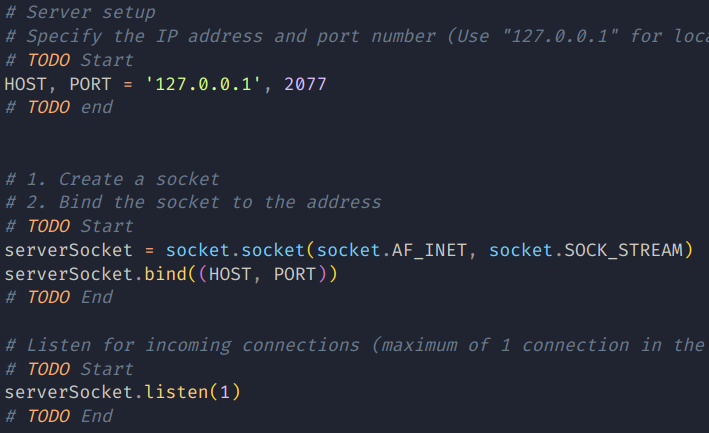
\includegraphics[width = 0.48\linewidth]{P2-1.png}    
    }\subfigure[accept the link from client]{
        \label{Fig.sub.2-2}
        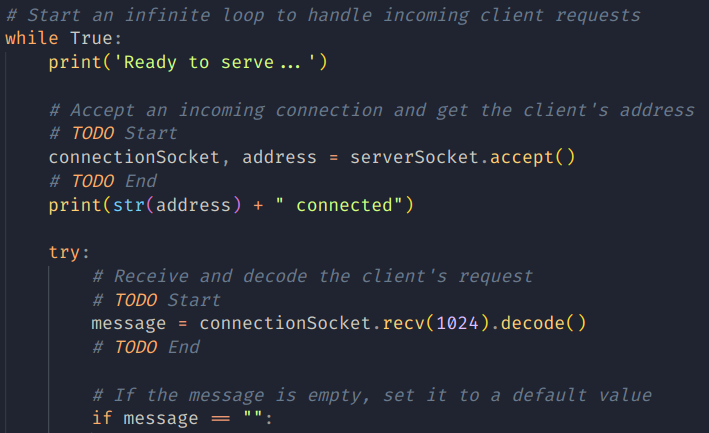
\includegraphics[width = 0.48\linewidth]{P2-2.png}
    }
    \subfigure[receive]{
        \label{Fig.sub.2-3}
        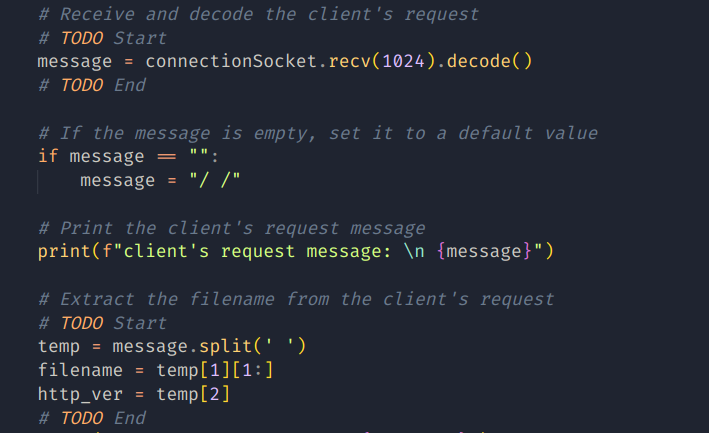
\includegraphics[width = 0.48\linewidth]{P2-3.png}
    }\subfigure[send HTTP response]{
        \label{Fig.sub.2-4}
        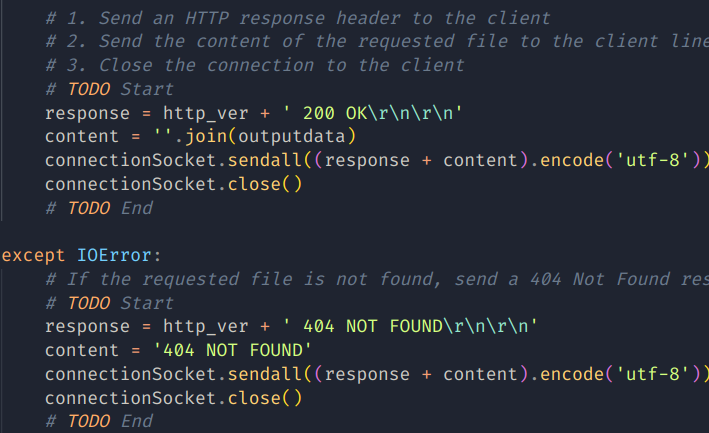
\includegraphics[width = 0.48\linewidth]{P2-4.png}
    }
    \caption{web\_server.py}
\end{figure}
\subsection{Result}
Here's the result of 2. 3. 4. in Figure 4.
\begin{figure}[H]
    \centering
    \subfigure[Access index.html]{
        \label{Fig.sub.2-6}
        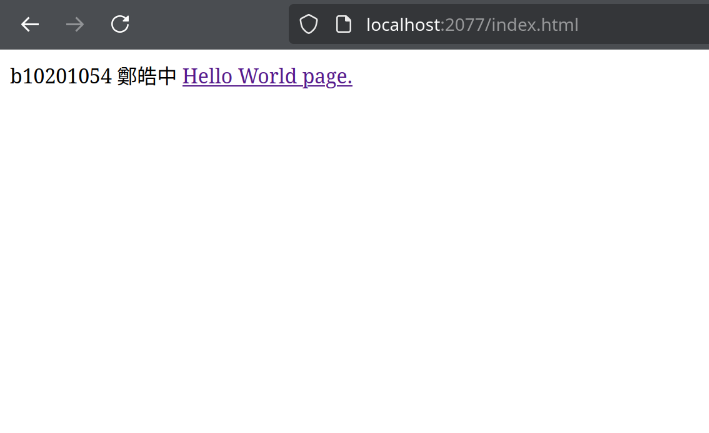
\includegraphics[width = 0.48\linewidth]{P2-6.png}    
    }\subfigure[Access index.html]{
        \label{Fig.sub.2-9}
        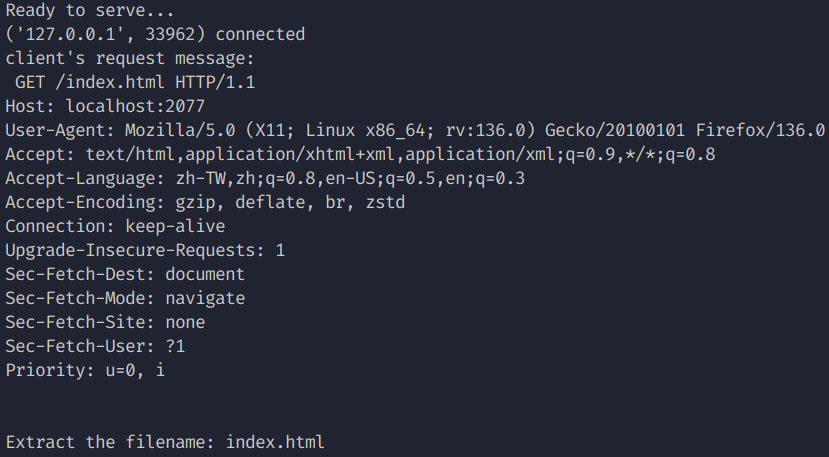
\includegraphics[width = 0.48\linewidth]{P2-9.png}
    }
    \caption{Access index.html}
\end{figure}
\begin{figure}[H]
    \subfigure[Access helloworld.html]{
        \label{Fig.sub.2-7}
        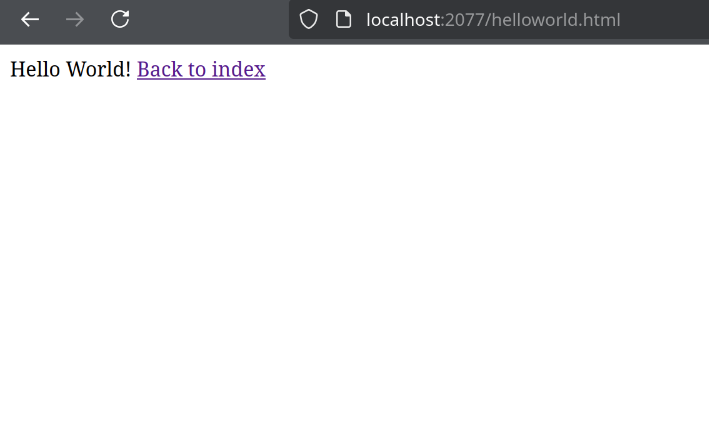
\includegraphics[width = 0.48\linewidth]{P2-7.png}
    }\subfigure[Access helloworld.html]{
        \label{Fig.sub.2-10}
        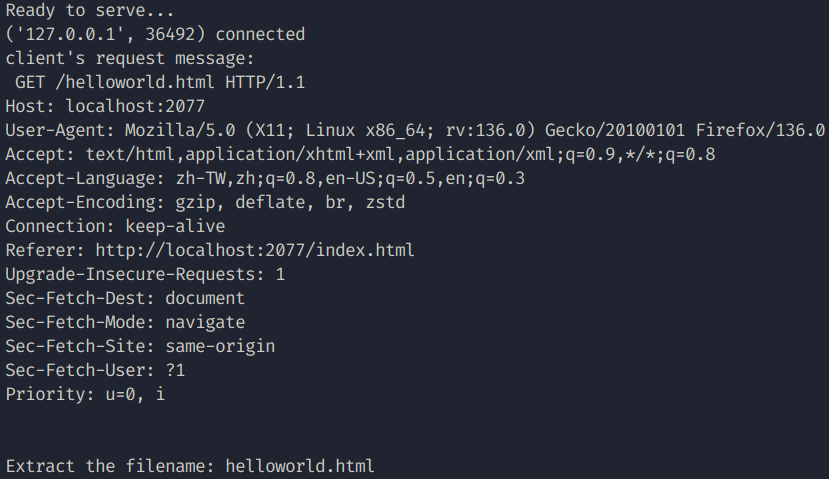
\includegraphics[width = 0.48\linewidth]{P2-10.png}
    }
    \caption{Access helloworld.html}
\end{figure}
\begin{figure}[H]
    \subfigure[Access testnotfound.html]{
        \label{Fig.sub.2-8}
        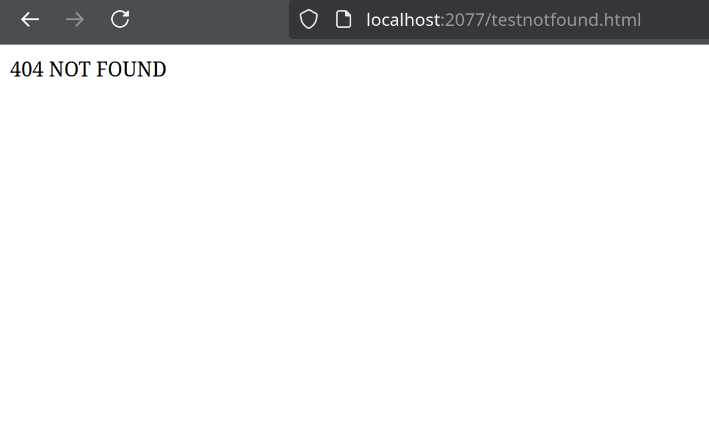
\includegraphics[width = 0.48\linewidth]{P2-8.png}
    }\subfigure[Access testnotfound.html]{
        \label{Fig.sub.2-11}
        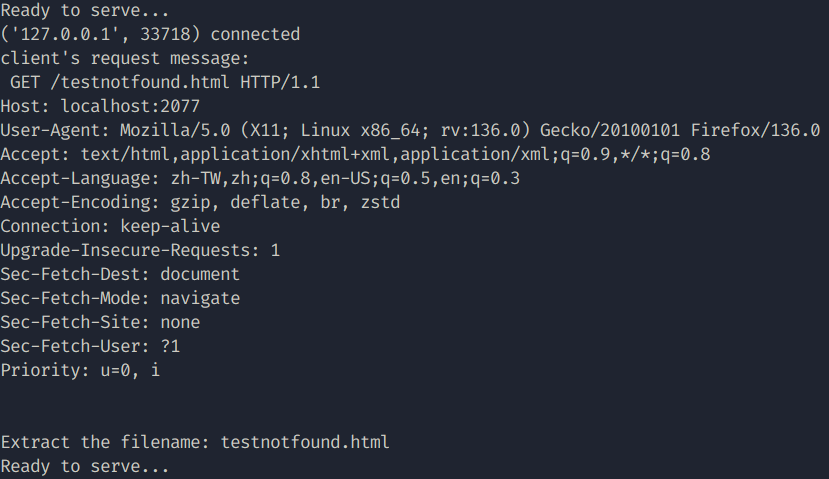
\includegraphics[width = 0.48\linewidth]{P2-11.png}
    }
    \caption{Access testnotfound.html}
\end{figure}
\newpage
\section{Proxy Server}    
\subsection{Code}
In the Figure 7.(a) and (b), it is same to setup socket and link.
In the Figure 7.(c), if we had already visited the page, it would be saved in cache, so that we can visit the page faster than asking web server again.
In the Figure 7.(d) and (e), if we hadn't visited the page yet, the proxy server would ask web server to get the data, then save the data in cache. 
If the web server HTTP response is 404, then don't cache anything since there is no data at web server.
\begin{figure}[H]
    \centering
    \subfigure[set HOST, PORT]{
        \label{Fig.sub.3-1}
        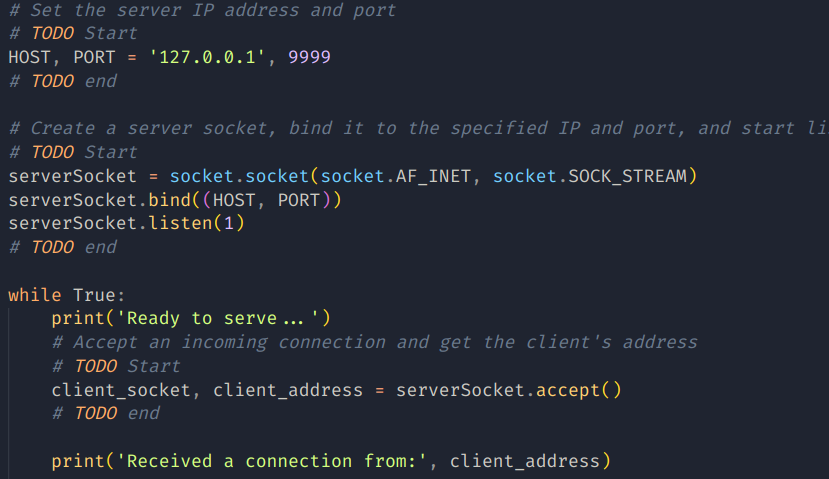
\includegraphics[width = 0.48\linewidth]{P3-1.png}    
    }\subfigure[accept the link from client]{
        \label{Fig.sub.3-2}
        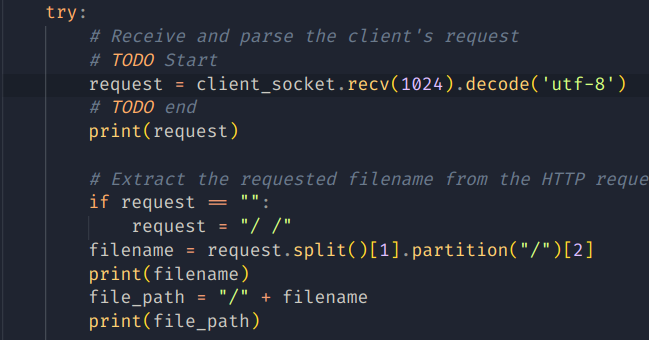
\includegraphics[width = 0.48\linewidth]{P3-2.png}
    }
    \subfigure[send and receive]{
        \label{Fig.sub.3-3}
        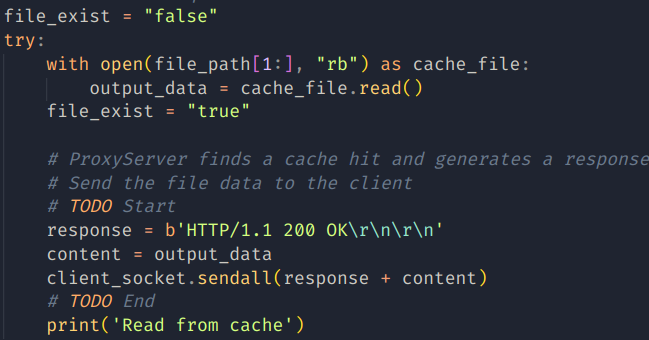
\includegraphics[width = 0.48\linewidth]{P3-3.png}
    }\subfigure[Final result at client side]{
        \label{Fig.sub.3-4}
        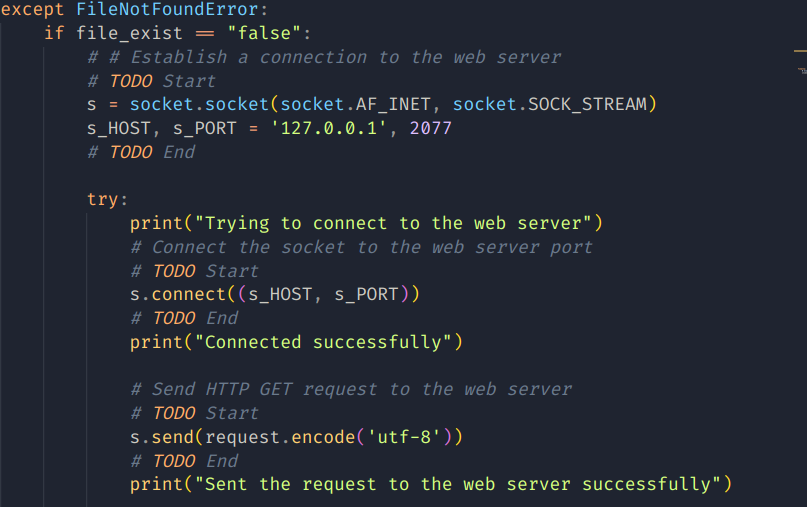
\includegraphics[width = 0.48\linewidth]{P3-4.png}
    }
    \subfigure[Final result at client side]{
        \label{Fig.sub.3-5}
        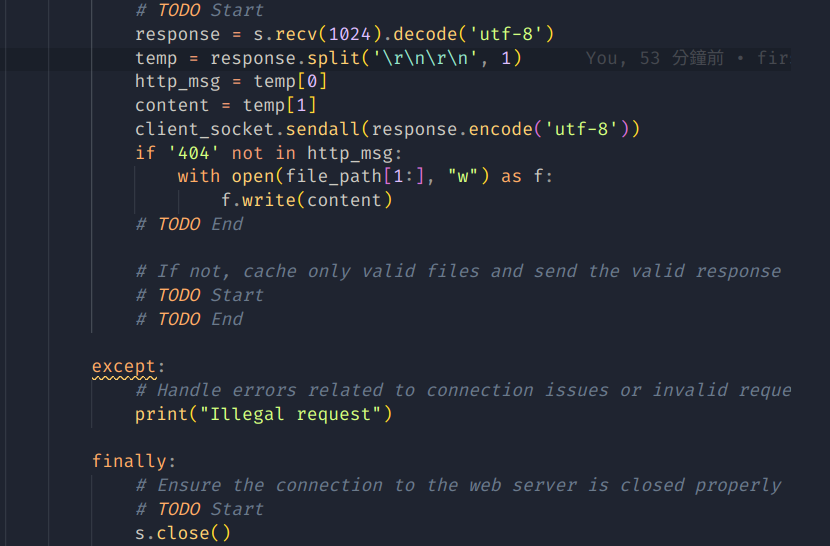
\includegraphics[width = 0.48\linewidth]{P3-5.png}
    }
    \caption{proxy\_server.py}
\end{figure}
\subsection{Result}

\begin{figure}[H]
    \centering
    \subfigure[Access index.html]{
        \label{Fig.sub.3-6}
        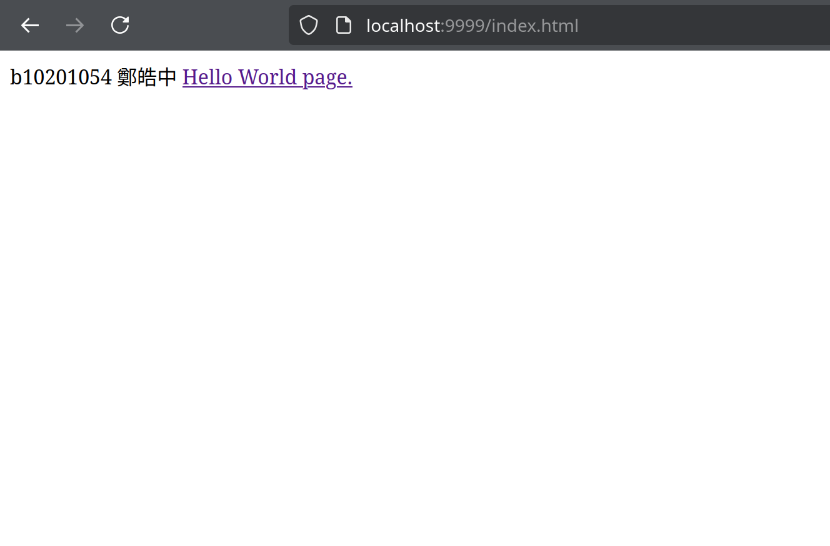
\includegraphics[width = 0.3\linewidth]{P3-6.png}    
    }\subfigure[Access index.html]{
        \label{Fig.sub.3-9}
        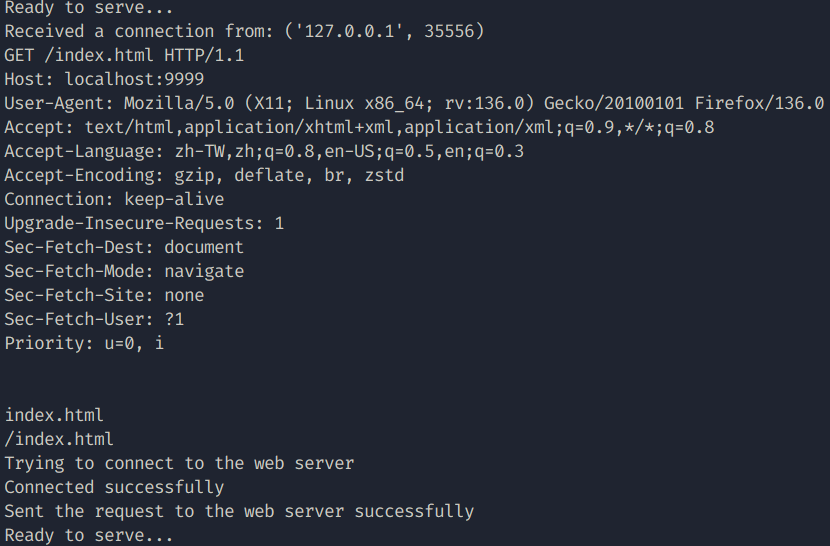
\includegraphics[width = 0.32\linewidth]{P3-9.png}
    }\subfigure[Access index.html]{
        \label{Fig.sub.3-12}
        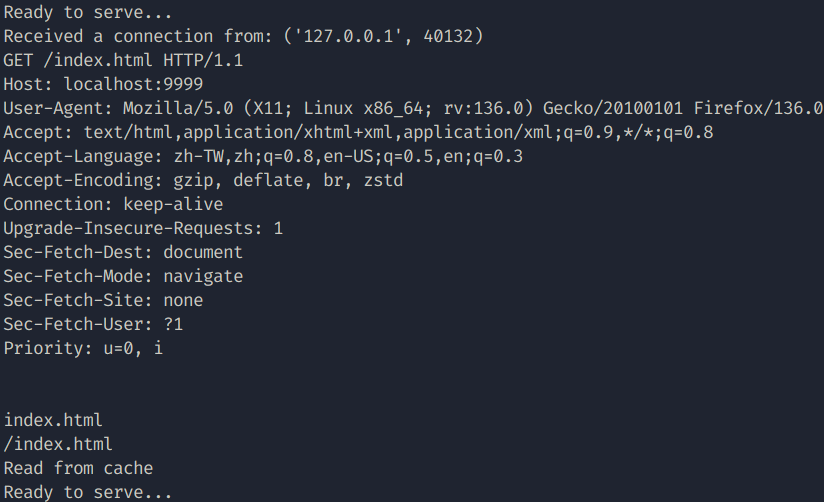
\includegraphics[width = 0.32\linewidth]{P3-12.png}
    }
    \caption{Access index.html}
\end{figure}
\begin{figure}[H]
    \subfigure[Access helloworld.html]{
        \label{Fig.sub.3-7}
        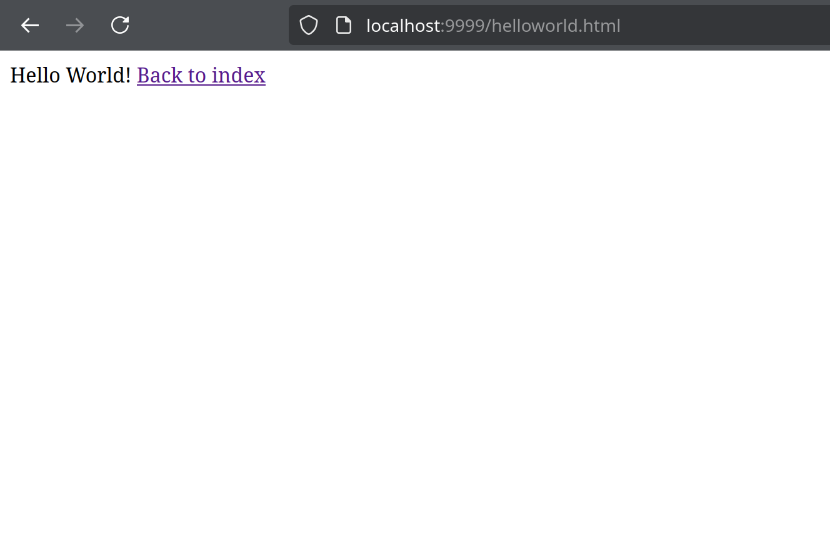
\includegraphics[width = 0.48\linewidth]{P3-7.png}
    }\subfigure[Access helloworld.html]{
        \label{Fig.sub.3-10}
        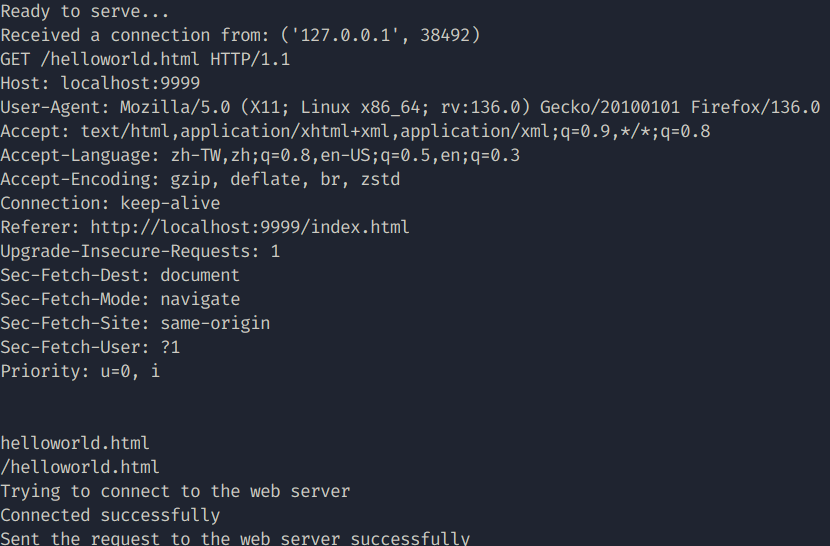
\includegraphics[width = 0.48\linewidth]{P3-10.png}
    }
    \caption{Access helloworld.html}
\end{figure}
\begin{figure}[H]
    \subfigure[Access testnotfound.html]{
        \label{Fig.sub.3-8}
        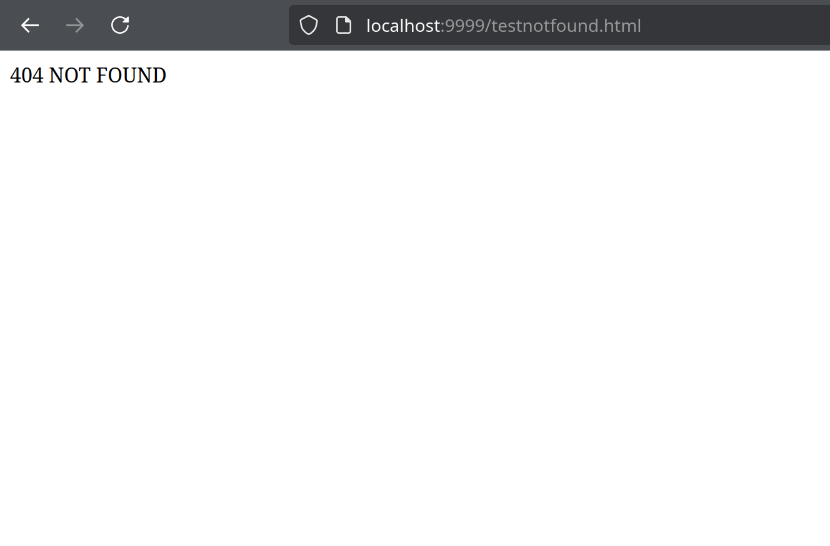
\includegraphics[width = 0.48\linewidth]{P3-8.png}
    }\subfigure[Access testnotfound.html]{
        \label{Fig.sub.3-11}
        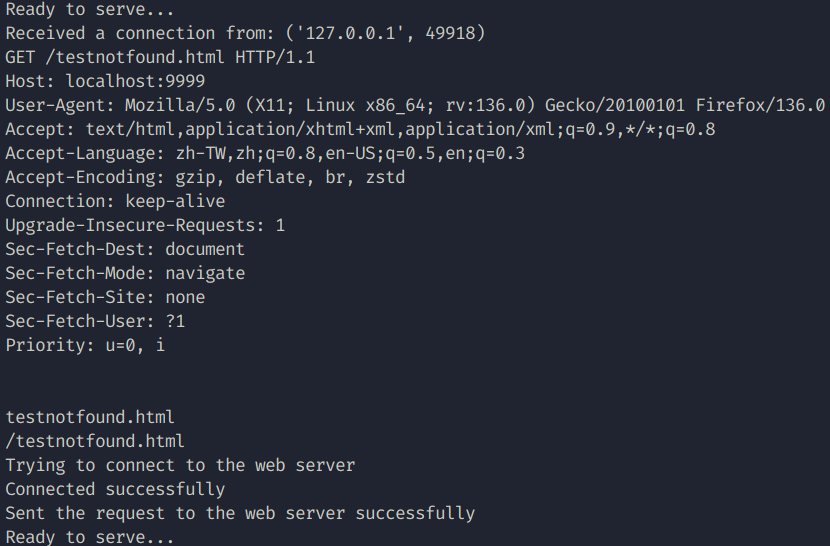
\includegraphics[width = 0.48\linewidth]{P3-11.png}
    }
    \caption{Access testnotfound.html}
\end{figure}
\end{document}
